\documentclass[man,floatsintext]{apa6}
\usepackage{lmodern}
\usepackage{amssymb,amsmath}
\usepackage{ifxetex,ifluatex}
\usepackage{fixltx2e} % provides \textsubscript
\ifnum 0\ifxetex 1\fi\ifluatex 1\fi=0 % if pdftex
  \usepackage[T1]{fontenc}
  \usepackage[utf8]{inputenc}
\else % if luatex or xelatex
  \ifxetex
    \usepackage{mathspec}
  \else
    \usepackage{fontspec}
  \fi
  \defaultfontfeatures{Ligatures=TeX,Scale=MatchLowercase}
\fi
% use upquote if available, for straight quotes in verbatim environments
\IfFileExists{upquote.sty}{\usepackage{upquote}}{}
% use microtype if available
\IfFileExists{microtype.sty}{%
\usepackage{microtype}
\UseMicrotypeSet[protrusion]{basicmath} % disable protrusion for tt fonts
}{}
\usepackage{hyperref}
\PassOptionsToPackage{usenames,dvipsnames}{color} % color is loaded by hyperref
\hypersetup{unicode=true,
            pdftitle={Catalan and Spanish natural speech segmentation at 8 months of age},
            pdfauthor={Gonzalo García-Castro, Mireia Marimon, Chiara Santolin, \& Nuria Sebastian-Galles},
            pdfkeywords={bilingualism, language acquisition, segmentation, phoneme learning, head-turn preference procedure},
            colorlinks=true,
            linkcolor=blue,
            citecolor=Blue,
            urlcolor=Blue,
            breaklinks=true}
\urlstyle{same}  % don't use monospace font for urls
\usepackage{graphicx,grffile}
\makeatletter
\def\maxwidth{\ifdim\Gin@nat@width>\linewidth\linewidth\else\Gin@nat@width\fi}
\def\maxheight{\ifdim\Gin@nat@height>\textheight\textheight\else\Gin@nat@height\fi}
\makeatother
% Scale images if necessary, so that they will not overflow the page
% margins by default, and it is still possible to overwrite the defaults
% using explicit options in \includegraphics[width, height, ...]{}
\setkeys{Gin}{width=\maxwidth,height=\maxheight,keepaspectratio}
\IfFileExists{parskip.sty}{%
\usepackage{parskip}
}{% else
\setlength{\parindent}{0pt}
\setlength{\parskip}{6pt plus 2pt minus 1pt}
}
\setlength{\emergencystretch}{3em}  % prevent overfull lines
\providecommand{\tightlist}{%
  \setlength{\itemsep}{0pt}\setlength{\parskip}{0pt}}
\setcounter{secnumdepth}{0}
% Redefines (sub)paragraphs to behave more like sections
\ifx\paragraph\undefined\else
\let\oldparagraph\paragraph
\renewcommand{\paragraph}[1]{\oldparagraph{#1}\mbox{}}
\fi
\ifx\subparagraph\undefined\else
\let\oldsubparagraph\subparagraph
\renewcommand{\subparagraph}[1]{\oldsubparagraph{#1}\mbox{}}
\fi

%%% Use protect on footnotes to avoid problems with footnotes in titles
\let\rmarkdownfootnote\footnote%
\def\footnote{\protect\rmarkdownfootnote}


  \title{Catalan and Spanish natural speech segmentation at 8 months of age}
    \author{Gonzalo García-Castro\textsuperscript{1}, Mireia Marimon\textsuperscript{2}, Chiara Santolin\textsuperscript{1}, \& Nuria Sebastian-Galles\textsuperscript{1, 3}}
    \date{}
  
\shorttitle{Segmentation}
\affiliation{
\vspace{0.5cm}
\textsuperscript{1} Center for Brain and Cognition, Pompeu Fabra University\\\textsuperscript{2} Department of Linguistics, University of Potsdam\\\textsuperscript{3} Department of Information and Communications Technologies, Pompeu Fabra University}
\keywords{bilingualism, language acquisition, segmentation, phoneme learning, head-turn preference procedure\newline\indent Word count: X}
\usepackage{csquotes}
\usepackage{upgreek}
\captionsetup{font=singlespacing,justification=justified}

\usepackage{longtable}
\usepackage{lscape}
\usepackage{multirow}
\usepackage{tabularx}
\usepackage[flushleft]{threeparttable}
\usepackage{threeparttablex}

\newenvironment{lltable}{\begin{landscape}\begin{center}\begin{ThreePartTable}}{\end{ThreePartTable}\end{center}\end{landscape}}

\makeatletter
\newcommand\LastLTentrywidth{1em}
\newlength\longtablewidth
\setlength{\longtablewidth}{1in}
\newcommand{\getlongtablewidth}{\begingroup \ifcsname LT@\roman{LT@tables}\endcsname \global\longtablewidth=0pt \renewcommand{\LT@entry}[2]{\global\advance\longtablewidth by ##2\relax\gdef\LastLTentrywidth{##2}}\@nameuse{LT@\roman{LT@tables}} \fi \endgroup}


\usepackage{lineno}

\linenumbers

\authornote{

Correspondence concerning this article should be addressed to Gonzalo García-Castro, 25-27, Ramon Trias Fargas, Barcelona 08005, Spain. E-mail: \href{mailto:gonzalo.garciadecastro@upf.edu}{\nolinkurl{gonzalo.garciadecastro@upf.edu}}}

\abstract{
Phoneme learning occurs in the first year of life when infants begin to acquire their first words. It is possible that infants use lexical-level information to identify relevant phonemes of their native languages. Since Catalan and Spanish are very lexically-similar languages, 8 months-old bilinguals represent an interesting population to investigate the possible top-down influence on phoneme learning. Catalan/Spanish bilinguals are typically exposed to higher vowel variability at the level of lexical representations with respect to their monolingual peers. For instance, infants seem to treat words like \emph{dodi} and \emph{dudi} similarly, despite being able to discriminate the /o/-/u/ contrast. The present research was aimed at investigating how Spanish/Catalan monolinguals and bilinguals encode new word forms at eight months when confronted with phoneme changes such as the aforementioned. We used an adaptation of Jusczyk and Aslin (1995)'s Head-turn Preference Procedure, which has proven to be suitable for investigating word-form learning in a wide variety of languages and ages. Infants were familiarized with sentences containing nonsense words in their native/dominant language. At test, we tested whether infants could identify familiar words presented individually along with novel words. We found no evidence of familair word recognition at test. Equivalence testing revealed that this outcome is unlikely to be drive by lack of statistical power. These results contrast with those obtained in previous studies reporting evidence of word segmentation using a similar with similar populations.


}

\begin{document}
\maketitle

\hypertarget{introduction}{%
\section{Introduction}\label{introduction}}

Language acquisition is a key milestone of infant development. One of the hallmarks of language acquisition is how effortlessly infants seem to achieve it, given its perceptual and structural complexity (e.g., Friederici, Chomsky, Berwick, Moro, \& Bolhuis, 2017). Speech is the first form of language to which infants are exposed, starting even before birth (Abboub, Nazzi, \& Gervain, 2016; DeCasper \& Spence, 1986; May, Byers-Heinlein, Gervain, \& Werker, 2011; Moon, Lagercrantz, \& Kuhl, 2013). After birth, infants must learn to identify and discriminate speech variations which are relevant for properly processing the language input. To do so, phoneme identification must be attained, as it is the simplest acoustic unit of speech. Different words are characterized by different phonemes. Hence, perception of such phonemes is a requirement to learn word forms, that is, to form new phonological representations and later be able to retrieve them to recognize the same words in different contexts.

From birth, infants bear sophisticated perceptual abilities that allow detections of subtle variations in the speech signal. These speech variations are more difficult to perceive later in life, when some of their perceptive abilities have adapted to the characteristics of the linguistic input. One of the domains that has been observed to be dependent of the speech input is phoneme learning, that is, the ability to discriminate and identify phonemic categories that exist in listeners' native language.

During the first six months of age, infants show a remarkable ability to differentiate both native and non-native phonemes without relevant experience (Dehaene-Lambertz and Dehaene (1994); Eimas, Siqueland, Jusczyk, and Vigorito (1971); Polka and Werker (1994); Werker and Tees (1984), Werker and Tees (2002){]}. From six to ten months, infants begin to lose this capacity and attune relevant feature of their speech input. This process, named perceptual narrowing, consists in a decline of the capacity to perceive non-native contrasts (e.g., Aslin, Pisoni, Hennessy, and Perey (1981); Werker and Tees (1984)). Non-prototypical phoneme productions (such as non-native phonemes) are perceived as the nearest prototypical native phoneme, in what has been named a perceptual magnet effect (Kuhl, Williams, Lacerda, Stevens, \& Lindblom, 1992). Those phonemes acoustically distant enough the native ones remain as indi- vidual categories, some of them as non-linguistic sounds (Best, McRoberts, \& Sithole, 1988). Werker, Gilbert, Humphrey, and Tees (1981) observed that six-to-seven month-old English learning infants were able to discriminate /Ta/-/ta/ and /th/-/dh/ Hindi-specific contrasts, whereas adults failed to do so in a similar task (see also Werker and Tees (1984)). Subsequent work replicated this developmental pattern using different consonant and vowel contrasts, namely: /r/-/l/ contrast in Japanese-learning infants (Kuhl et al. (1992)), Hebrew /b/-/p/ contrast in Arabic-learning infants (Segal, Hejli-Assi, \& Kishon-Rabin, 2016), /t\(\int\)h/-/t\(\int\)/ Urdu contrast in English-learning infants (Dar, Keren-Portnoy, \& Vihman, 2018), /U/-/Y/ and /u/-/y/ German vowel contrasts in English-learning infants (Polka \& Werker, 1994), or /e/-/e/ vowel contrast in Spanish learners (Bosch \& Sebastian-Galles, 2003).

Perceptual narrowing is not the only process involved in phonemic learning. Attunement to native speech also seems to provide an enhanced sensitivity to phonemic contrasts characterizing native languages (Kuhl et al., 2006; Polka, Colantonio, \& Sundara, 2001; Shin, Choi, \& Mazuka, 2018; Tsuji \& Cristia, 2014). Moreover, some studies have found remarkable variability in the developmental pattern of different phonemes. For instance, Best and McRoberts (2003), Best, McRoberts, and Goodell (2001), and Best, McRoberts, LaFleur, and Silver-Isenstadt (1995) observed that some non-native contrasts prevail perceptual narrowing, while several cross-linguistic studies showed directional asymmetries in infant vowel perception, that is, some are more difficult to perceive when its phonemes are presented in a particular order (Dar et al., 2018; Kuhl et al., 2006; Polka \& Bohn, 1996; Segal et al., 2016).

Thus, phoneme learning seems to be a quite complex mechanism determined by the combination of distinct processes. Yet, the aforementioned results suggest that, by the end of the first year, infants possess a phonemic inventory specific to the language(s) they are exposed the most. What cues do infants rely on to warp their phonemic inven- tory, and whether they differently use these cues at different points in development remain some elusive issues. Since the speech signal provides several types of information that are available to the infant during speech perception, previous research has investigated the potential exploitation of such cues by the infants to bootstrap phonemic categories.

Most of the mechanisms suggested to account for phoneme learning can be linked to a bottom-up approach. One of such mechanism is the distributional account, according to which six-to-eight-month-olds consider the relative frequency of a given phoneme as the principal cue in order to discover native phonemic contrasts (see Saffran \& Kirkham, 2018 for a review). In particular, Maye, Werker, and Gerken (2002) found that six-to-eight month-olds showed a decline in discrimination of the /da/-/ta/ contrast after exposure to an unimodal distribution of the two phonemes. This means that participants found more difficult to perceive such contrast when most of the previous realizations of each phoneme lied at the center of the acoustic \emph{continuum} formed by the /da/ and /ta/ extremes. Conversely, infants exposed to a bimodal distribution (most of the realizations lied in the extremes of the \emph{continuum}, corresponding to the \enquote{prototypical} /da/ and /ta/) not only showed discrimination, but also a facilitation effect of the aforementioned contrast (Maye, Weiss, \& Aslin, 2008). At 10 months, infants seemed to be less sensitive to the distributional properties of their linguistic input (Yoshida, Pons, Maye, \& Werker, 2010), a fact that might reveal the existence of a critical period (in between six and eight months) during which infants make particular use of statistical properties of the speech to detect phonemes. According to the distributional account, after this perceptual narrowing, less fre- quent phonemes would fall into the acoustically closest category formed by high frequent phonemes. Hence, distributional properties embedded in the speech signal might provide valuable information about how relevant a phoneme is when perceiving native language. Despite statistical learning has provided an interesting framework to study phoneme learning, subsequent research has shown that distributional information might not be sufficient to guide this process, and that other processes may play an important role in determining native phonetic inventory.

Some of the distributional account's predictions have been challenged by the results obtained in bilingual populations. In particular, Bosch and Sebastian-Galles (2003) observed Catalan/Spanish bilingual infants, and found a U-shaped developmental pattern concerning the /e/-/\(\varepsilon\)/ Catalan vowel contrast. Bilinguals and Spanish and Catalan monolinguals were able to discriminate this contrast at four months but not at eight, when only Catalan monolinguals showed discrimination. Surprisingly, bilinguals showed no discrimination when the /e/ and /\(\varepsilon\)/ vowels were interchanged, just like Spanish monolinguals did. In addition, at 12 months, bilingual infants regained discrimination. Given that Catalan-Spanish bilinguals were exposed to the /e/-/\(\varepsilon\)/ just like Catalan monolinguals, these results posed a challenge to the assumption that mere exposure to native lan- guages is sufficient to drive infants into native phonemic systems.

Distributional learning can, potentially, explain the U-shaped pattern found by Bosch and Sebastian-Galles (2003). The Spanish /e/ lies in between the Catalan /e/ and /\(\varepsilon\)/ in the acoustic space, and is much more frequent than the latter (30\% in Spanish versus 8\% in Catalan Alcina, Franch, \& Blecua, 1979; Rafel, 1979). Hence, bilinguals might have been exposed to a unimodal-like distribution of the contrast. In distributional terms, this would mean that bilinguals may have been exposed much more frequently to the Spanish /e/ than to the Catalan /e/ and /\(\varepsilon\)/ vowels. In line with Maye et al. (2002), discrimination of the Catalan contrast might have been hindered by exposure to the unimodal distribution underlying the bilingual input. Later recovery of discrimination was explained by the authors by cumulative experience of bilingual infants to each of the languages. Indeed, it is important to mention that the typical amount of individual language exposure of bilingual infants is lower than that of monolinguals. Bosch and Sebastian-Galles (2003) pointed that bilinguals might take longer to reach the same level of acoustic experience. However, given that at 12 months the distributional properties of the speech input are likely the same, it is possible that mere exposure to them is not sufficient to regain this contrast at this age.

The underlying assumptions of the distributional account were challenged by subsequent research. Sebastian-Galles and Bosch (2009) found the same U-shaped developmental pattern in Catalan/Spanish bilinguals using another vowel contrast, /o/-/u/, present in both languages. Unlike the /e/-/\(\varepsilon\)/ contrast, the /o/-u/ contrast is present in both Catalan and Spanish and accommodates better a bimodal distribution. As indicated by Sebastian-Galles \& Bosch, the /o/ vowel is more frequent that the /u/ vowel in Spanish, while the /u/ vowels is more frequent than the /o/ vowel in Catalan. Nonetheless, the acoustic region of each phoneme is clearly separated. Following the distributional account, infants should have distinguished this bimodal-like contrast at all ages. Bilinguals, however, again failed at discriminating this contrast at eight months. Additionally, when tested with the /e/-/u/ contrast (bimodal but acoustically more distant), bilinguals' developmental pattern matched that showed by Catalan monolinguals. Figure 1 illustrates the distributional account's predictions and the results obtained in Catalan/Spanish mono- linguals and bilinguals.Altogether these results show that the distributional learning account may not be sufficient to explain phonemic learning in bilingual contexts.

\begin{figure}
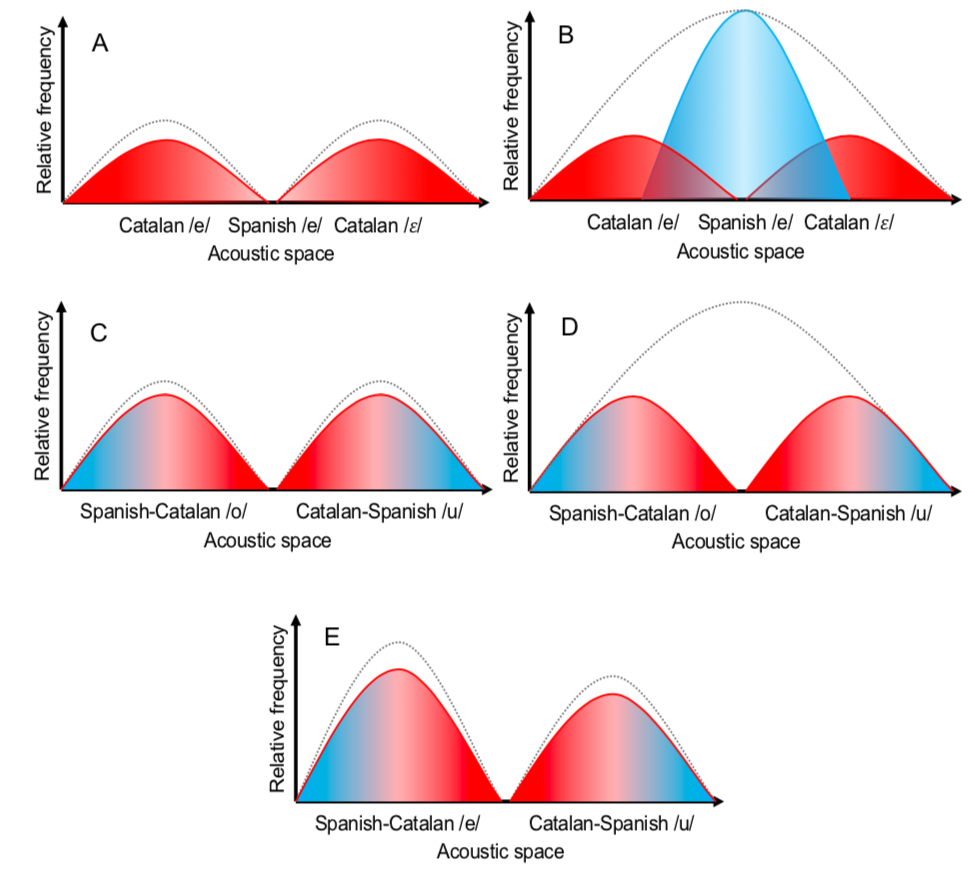
\includegraphics[width=1\linewidth]{/Users/GonzaloGGC/projects/Segmentation/Figures/vowel_distributions} \caption{Distributional account's predictions and evidence. Catalan and Spanish phonemes in red and blue, respectively. The dashed line represents the resultant phonetic category as predicted by the distributional account. A) Catalan monolinguals were predicted to form distinct categories for the /e/ and /e/ Catalan vowels. Accordingly, they showed discrimination of the /e/-/e/ contrast. B) Catalan/Spanish bilinguals were predicted to merge the Catalan /e/ and /e/ and the Spanish /e/ vowels into the same category. Accordingly, they did not show discrimination. C) Catalan/Spanish bilinguals were predicted to form distinct categories for the /o/ and /u/ Catalan and Spanish vowels. D) No discrimination was shown in the /o/-/u/ contrast, which might indicate that they were also merged into the same category, contrary to what predicted. E) However, the /e/-/u/ contrast, which bears a similar distribution than the /o/-/u/ contrast, was discriminated.}\label{fig:unnamed-chunk-1}
\end{figure}

On the other hand, results by Albareda-Castellot, Pons, and Sebastian-Galles (2011) using an anticipation paradigm showed that discrimination of the /e/-/\(\varepsilon\)/ contrast does take place at 8 months in bilinguals, and suggested that the previous results might be due to a lack of saliency/attention rather than to a discrimination at this age. Sebastian-Galles and Bosch (2009) and also Albareda-Castellot et al. (2011) suggested that the existence of a high number of cognates between Spanish and Catalan resulted in a difference in the pattern of responses between monolinguals and bilinguals in paradigms requiring recovery of attention in the test phase.

As noted by Sebastian-Galles and Bosch (2009), Catalan and Spanish bear high phono-lexical similarity. This can be illustrated by the fact that cognates -- words that share an etymological origin, hence, phonological similarity -- represent over 65-70\% of the lexical inventory of both languages (Green, 1988). Spanish-Catalan cognates frequently differ in acoustically close vowels, often involving exchanges of phonemes from the /e/-/\(\varepsilon\)/ and /o/-/u/ vowel contrasts (e.g. {[}o.'\(\beta\)e.xa{]}, \emph{sheep} in Spanish changes to {[}u.ˈ\(\beta\)e.ʎa{]} in Catalan). This fact results into a larger exposure to vowel variability at the level of lexical representations in Catalan/Spanish bilingual infants with respect to their monolingual peers. For this reason, such bilinguals might disregard vowel changes involving the /e/-/\(\varepsilon\)/ and /o/-/u/ vowel contrasts that occur in similar word contexts (i.e., cognates). Supporting this hypothesis, Ramon-Casas, Swingley, Sebastian-Galles, and Bosch (2009) found that Catalan/Spanish bilinguals show lower sensitivity to vowel mispronunciations within cognates involving the /e/-/\(\varepsilon\)/ contrast, while other studies showed that bilinguals are still able to discriminate such contrast when presented in minimally differing words (Ramon-Casas, Fennell, \& Bosch, 2017).

The aforementioned studies provide support for this hypothesis: infants discriminate both contrasts (Albareda-Castellot et al., 2011), but do not seem to change their response pattern when confronted with /e/-/\(\varepsilon\)/ and /o/-/u/ vowel switches (Bosch \& Sebastian-Galles, 2003; Sebastian-Galles \& Bosch, 2009). This could indicate that Catalan-Spanish infants consider /e/-/\(\varepsilon\)/ and /o/-/u/ vowel switches as irrelevant when encoding new word forms. In other words, lexical-level information might modulate phoneme learning at 8 months.

Phoneme learning models have traditionally omitted the fact that infants are rarely exposed to isolated phonemes. Rather, the phonemic inventory to which they must attune is embedded in words. According to a complementary approach, the cues that might guide phonemic learning might also be encoded in the lexical level, involving top-down mechanisms. Word-level information is already available to infants from six to 12 months (Bergmann \& Cristia, 2016), the same age range during which phonemic perceptual narrowing develops. As suggested by previous studies, lexical knowledge could guide infants in tuning into native-language(s)' phoneme inventory, possibly interacting with bot- tom-up-guided processes (Elsner, Feldman, \& Wood, 2013).

Evidence from simulated data has provided several hypotheses on what type of cues may lead to successful phonemic learning, and how should these cues be weighted in order to best attune to the acoustic input provided by the speech signal. Distributional learning seems to explain phonemic learning just partially, since successful classification rates in computational models are lower when phonetic categories overlap in the acoustic space (Dillon, Dunbar, \& Idsardi, 2013) regardless of the amount of distributional information provided. In contrast, using Bayesian models, it has been suggested that lexical cues seem to provide additional information regarding phonetic classification, potentially playing a central role in phonemic learning (Feldman et al., 2013a). The same results have been shown in

Eight-month-old infants and adults (Feldman et al., 2013b). In summary, hearing acoustically similar phonemes in distinct word contexts could lead to the formation of separate phonetic categories. If the distributional properties of the speech input were sufficient for bootstrapping phonetic categories, lexical information should be redundant. The results observed by Feldman et al., however, suggest that lexical information could indeed be critical for successfully for phonetic categories. The lexical account provides valuable insights for revisiting bilingual phonemic learning.

Infants begin to create word forms between six to twelve months of age. The seminal works by Jusczyk and Aslin (1995); Jusczyk, Houston, and Newsome (1999) revealed that infants start segmenting speech (i.e., extracting words forms from the speech stream) of native language at 8 months of age. Using the Head-turn Preference Procedure, 6- to- 7- month-olds were familiarized to individual monosyllabic words. The same words and other new words were presented embedded in sentences at test. Results showed that only 7-month-olds were able to distinguish familiar vs.~unfamiliar words, suggesting that they segmented the target words from the sentences. Additionally, they examined how acoustically detailed was the representation of word forms. Infants were tested with the same words, but some of them had been changed in one consonantal phoneme. Infants treated these new words as unfamiliar, what suggested that infants at 7 months of age are able to represent acoustically accurate word forms. Importantly, these early segmentation abilities have been shown in different languages (e.g. Nishibayashi, Goyet, \& Nazzi, 2015) as well as in bilingual infants (Bosch, Figueras, Teixidó, \& Ramon-Casas, 2013).

Segmentation appears to be guided by different cues contained in the speech signal, which are used differently based on infants' linguistic experience. For instance, statistical distributions of syllables composing words (e.g., co-occurrence frequencies, transitional probabilities) are privileged around 8 months of age to detect individual words embedded in an artificial language with no other cues to word boundaries (e.g., Saffran, Aslin, \& Newport, 1996; Saffran \& Kirkham, 2018; Santolin \& Saffran, 2018 for review). In addition to statistical cues, prosodic information helps infants to segment the speech. Neonates are already sensitive to some suprasegmental features of the speech stream (Abboub et al., 2016; Bertoncini, Floccia, Nazzi, \& Mehler, 1995; Christophe, Mehler, \& Sebastian-Galles, 2001), and this rhythm perception is later attuned to match the native language input (Bhatara, Boll-Avetisyan, Unger, Nazzi, \& Höhle, 2013; Skoruppa et al., 2013). Both statistical and suprasegmental cues, along with others, such as phonotactics (Friederici \& Wessels, 1993; Gonzalez-Gomez \& Nazzi, 2013; Sebastian-Galles \& Bosch, 2002), contribute to the extraction of word forms from speech, based on the prop- erties characterizing different languages (Thiessen \& Saffran, 2003).

Most of the literature agree in that early speech segmentation is partially sup- ported by bottom-up mechanisms however, as lexical processes take place and infants develop word forms, bottom-up and top-down mechanisms interact in speech segmentation (Jusczyk et al., 1999; Mersad \& Nazzi, 2012). Indeed, lexical processes may help infants with additional information necessary to segment the speech, especially when the input does not provide enough cues to word boundaries. Furthermore, it has been suggested that, if infants are able to recognize words within the speech stream, it is likely the case that phonological representations of words bootstrap phonemic learning.

In short, it has been proposed that 1) infants must first learn phonemes to later identify word forms, and 2) lexical-level information may influence phoneme learning at the same time. For example, 8-month-old Catalan/Spanish bilinguals ignore switches of contras- tive vowels within words, namely the /e/-/\(\varepsilon\)/ and the /o/-/u/ vowels. Catalan/Spanish bilinguals are exposed these switches within similar word contexts, provided by cognates. This could be leading them to store a common phonological representation for both realizations of the cognate, hence, to ignore such phoneme variability. If this is true, it could be predicted that, after segmentation, if the /e/ and /\(\varepsilon\)/ or the /o/-/u/ vowels are interchanged in familiar words, the resulting words would still be treated as familiar. Conversely, if the change implicates a contrast that is less commonly involved in cognates such as the /e/-/u/ or a consonant contrast, it would lead to the resulting words to be treated as unfamiliar by 8 months-old Catalan/Spanish bilinguals, as Jusczyk and Aslin (1995) found.

In summary, the main objective of the present research would be to investigate whether bilingual infants show the same response pattern than monolinguals when presented with a vowel change involving the /o/-/u/ and the /e/-/u/ contrasts. In order to investigate this issue, it must be first verified that we use a paradigm that results in segmentation at 8 months by Catalan-Spanish monolinguals and bilinguals. Therefore, the present study represents a control study aiming at testing the procedure and acquiring a baseline with which compare results provided by the manipulation of the acoustic materials (e.g.~using different phonemic contrasts) in subsequent experiments. To investigate segmentation abilities in 8 months-old infants, we will use the Head-turn Preference Procedure, as in Jusczyk and Aslin (1995). This procedure allows to test discrimination amongst acoustic stimuli through visual preferences, assessing whether infants look longer to visual objects associated to familiar and unfamiliar acoustic stimuli. Many pitfalls have been raised concerning the interpretation of results provided by this paradigm. However, it is a highly used procedure that has proved to be a suitable para- digm to test segmentation abilities in both monolinguals and bilinguals (e.g. Bosch et al., 2013; Goyet, Nishibayashi, \& Nazzi, 2013; Jusczyk et al., 1999).

In this experiment, infants will be familiarized with non-words embedded in real sentences; at test, isolated target words will be presented along with unfamiliar words, and discrimination will be measured. Different looking times associated with familiar and unfamiliar test words would indicate recognition of words heard during familiarization; hence that infants have successfully parsed the speech stream and identified the target words. Moreover, this would likely suggest that phonological representations of words are available for bootstrapping of phoneme categories.

Stimuli will consist of non-words to avoid potential previous familiarity with the speech material. In the familiarization phase, non-words (from now, target words) will be embed- ded in sentences either in Catalan or in Spanish (depending on the dominant language of the infant). At this age, infants show difficulties to segment polysyllabic words (Jusczyk et al., 1999; Nishibayashi et al., 2015). Thus, we will use monosyllabic non-words. Infants will be familiarized with different CVC monosyllabic target words, one of them containing the /o/ vowel, and other containing the /u/ vowel. As highlighted previously, the /o/-/u/ contrast is not only present in both Catalan and Spanish, but also it accommodates a bimodal distribution in the acoustic space, that is, both phonemes are frequent in each language. Moreover, in procedures based on recovery of attention, bilinguals do not show changes in their response patterns at 8 months-of age when confronted with switches involving this contrast. This makes this contrast ideal for the aim of present study. Bosch et al. (2013) have previously shown that Catalan/Spanish bilinguals were able to segment monosyllables from sentences. However, the stimuli they used did not involve the /o/-/u/ contrast, and thus did not allow to test the current hypothesis. Subsequent experiments will test whether either a vowel (e.g. /o/ for /u/) or a consonant change (e.g. /f/ for /b/) might exert an effect on infants looking times to familiar or unfamiliar words, what may reveal how flexible are the potential phonological representation of target words created by infants, and whether this flexibility is present in both vowels and consonants according to the speech input that they receive.

Previous research had shown that infants at 8 months of age listen longer to the familiar materials, indicating familiarity preference in both monolinguals (e.g., Jusczyk \& Aslin, 1995; Nazzi, Dilley, Jusczyk, Shattuck-Hufnagel, \& Jusczyk, 2005; Nishibayashi et al., 2015) and bilinguals (Polka, Orena, Sundara, \& Worrall, 2017). However, Bosch et al. (2013) found an inverse pattern when testing Catalan- and Spanish-learning mon- olinguals and bilinguals: both infants looked longer to novel words at 8 months of age. The interpretation of preferences is not straightforward, since many factors play a role in the directionality of the preferences (Houston-Price \& Nakai, 2004). It has been claimed that familiarity-novelty preference is dependent of the proficiency of the participants in speech perception: more proficient infants would show a novelty preference while less proficient ones would show a familiarity preference. Bosch et al. (2013) interpreted the novelty preference they found in 8 months old bilinguals as an indicator of such profi- ciency, since 6-month-olds showed a familiarity preference. However, not only age influences the preference, as a recent meta-analysis has shown (Bergmann \& Cristia, 2016). Also other factors, such as time a familiarization during the procedure might exert an effect on the directionality of preference (Hunter \& Ames, 1988). Since the novelty-pref- erence found by Bosch et al.~is not consistent with the direction of preference reported by previous studies, we will also analyze the preference that the infants of the present study.

\hypertarget{methods}{%
\section{Methods}\label{methods}}

\hypertarget{participants}{%
\subsection{Participants}\label{participants}}

We collected data from 36 full-term 8-month-old infants (17 females) with no history of hearing, motor, or vision problems according to parents' report. The accepted age range for collecting participants was from 7;15 to 9 months (261-280 days). Participants were recruited from private clinics in the Metropolitan area of Barcelona (Spain). Informed consent was obtained prior to any procedure. Socioeconomic status and linguistic environment were assessed using a detailed questionnaire as in Bosch and Sebastian-Galles (2001). Infants with equal or longer exposure than 80\% of the total time to one of their languages were considered monolinguals while those exposed less than 80\% of the total time to one of their languages were considered bilingual.

Twenty-one monolinguals (Mean age = 250.52 days, range = 228-276 days) from monolingual Catalan (\emph{n} = 14) and Spanish (\emph{n} = 7) environments, and 15 bilinguals (Mean age = 256.20 days, range = 229-271 days), from Catalan-dominant (\emph{n} = 9) and Spanish-dominant (\emph{n} = 6) environments were included in the final analysis. Mean exposure to dominant language was 94.29\% (range = 80-100\%) in the Catalan monolingual group, 92.71\% (range = 85-100\%) in the Spanish monolingual group, 70.56\% (range = 50-100\%) in the Catalan-dominant bilingual group, and 92.71\% (range = 85-100\%) in the Spanish-dominant bilingual group. Fifteen additional participants were excluded due to health-related issues (\emph{n} = 4), unsuitable linguistic profile (\emph{n} = 4), experimental failure (\emph{n} = 3), failure to reach the minimum number of 8 valid test trials (\emph{n} = 2), no reaching the test phase (\emph{n} = 1), or parental interference (\emph{n} = 1). Parental educational attainment is presented in Appendix 1.

\hypertarget{stimuli}{%
\subsection{Stimuli}\label{stimuli}}

We used four target non-words: \emph{gon}, \emph{mus}, \emph{for}, and \emph{pul}, taken from Marimon (2015). Half of the words contained the /o/ phoneme (\emph{gon}, \emph{for}) and the other half contained the /u/ phoneme (\emph{mus}, \emph{pul}), both contrastive in Catalan and Spanish. None of those words exist in Spanish\footnote{The word \emph{mus} actually exists. It is a card game. However, infants are extremely unlikely to be familiar with this word.}. All word phonemic onset involved a consonant, as infants have been shown to start segmenting words starting with consonants earlier than words starting with vowels (Mattys \& Jusczyk, 2001). We created six different sentences for each target word. The position of the target word within the sentences was counterbalanced so every passage grouped sentences containing the target words at the initial (2), middle (2) and final (2) positions.

\hypertarget{stimuli-recording-and-editing}{%
\subsubsection{Stimuli recording and editing}\label{stimuli-recording-and-editing}}

For each word we created 7 different passages combining the same 6 sentences, separated by 1 second. Within each passage, the order of the sentences was randomised using a randomizer (\url{www.random.org}). The sentences were concatenated in random order with one constraint: the last sentence of one passage should not be the same as the first of the next passage, to avoid the same sentence to be repeated consecutively. The order of the resulting passages was the same in both languages. The passages were presented in the same order to all infants in the same condition.

Natural exemplars of each word were produced by a highly competent Catalan/Spanish bilingual female and recorded in a sound attenuated room with a multi-pattern condenser microphone. The talker was asked to read the stimuli while not emphasizing the target non-words. The same talker recorded all stimuli in a single session. Words were digitized, down-sampled to 16 KHz and edited using Praat 6.0.37 (Boersma \& Weenink, 2018) and Audacity software (version 2.0.5; Team (2018)\footnote{Audacity® software is copyright © 1999-2018 Audacity Team Web site: \url{https://audacityteam.org/}. It is free software distributed under the terms of the GNU General Public License. The name Audacity® is a registered trademark of Dominic Mazzoni.}), saved as \texttt{.wav} files, and finally edited using Praat (version 6.0.37; Boersma \& Weenink, 2018). The edition pipeline for the passages consisted in the following steps: 1) Sentences were recorded (online monitoring ensured good sound quality recording), 2) silences at the onset and the offset of each recording were removed, 3) peak intensity intensity for each passage was normalised at 65.0 dB, 4) silences of 1000 ms duration were added at the offset of each recording, 5) sentences embedding the same word were concatenated, 6) passages of each condition were concatenated. This step resulted in four different strings: a \emph{gon-mus} string in Catalan, a \emph{gon-mus} string in Spanish, a \emph{for-pul} string in Catalan, and a \emph{for-pul} string in Spanish. Within each condition, all infants listened to the same string.

The edition pipeline for the \textbf{test words} consisted on the following steps: 1) Words were recorded individually exactly as sentences were recorded, by the same speaker, in the same session, 2) silences at the onset and the offset of each recording were removed, and 3) peak intensity of each passage was normalised at 65.0 dB. The spaces between words in the test phase was introduced by the script used to display stimuli during the experiment.

\hypertarget{procedure}{%
\subsection{Procedure}\label{procedure}}

An adaptation of the Head-turn Preference Procedure was used to test whether infants segmented the target words from the sentences as in Jusczyk and Aslin (1995), and Bosch and Sebastian-Galles (2003)). Figure 2 illustrates the set up used for testing infants. Infants sat on parent's lap in a sound-attenuated room equipped with three computer screens placed in front of, and on the two sides of the infant. The experimenter remained in an adjacent testing booth, blind to the audio stimuli (hence to the experimental condition) and coded on-line looking times using custom-designed MATLAB software (R2017b, MathWorks, Inc.; WISP - Wisconsin Infant Studies Program by Rob Olson \& Jenny Saffran, UW-Madison).

Infants were familiarized with one of the two passages (based on participants' dominant language) for two minutes; during the first minute infants heard the stimuli and watched to moving clouds presented on the central screen. During the second minute, a blinking light was displayed contingent on infant looking behavior to familiarize infants with the experimental setting. After familiarization, there were 12 test trials, three for each of the four test items, presented in random order. At the beginning of each test trial, a pinwheel was displayed on the central screen until the infant fixated on it. At that point, the experimenter signaled the central pinwheel to extinguish and one of two side-pinwheels to pop up. When infants looked at the side pinwheel, one of the target words (either one of the two familiar or unfamiliar words) was played repeatedly, with 1,500 ms in between each repetition until the infant looked away for 2,000 ms, or until cumulative 17,000 ms of looking time had elapsed.

\begin{figure}
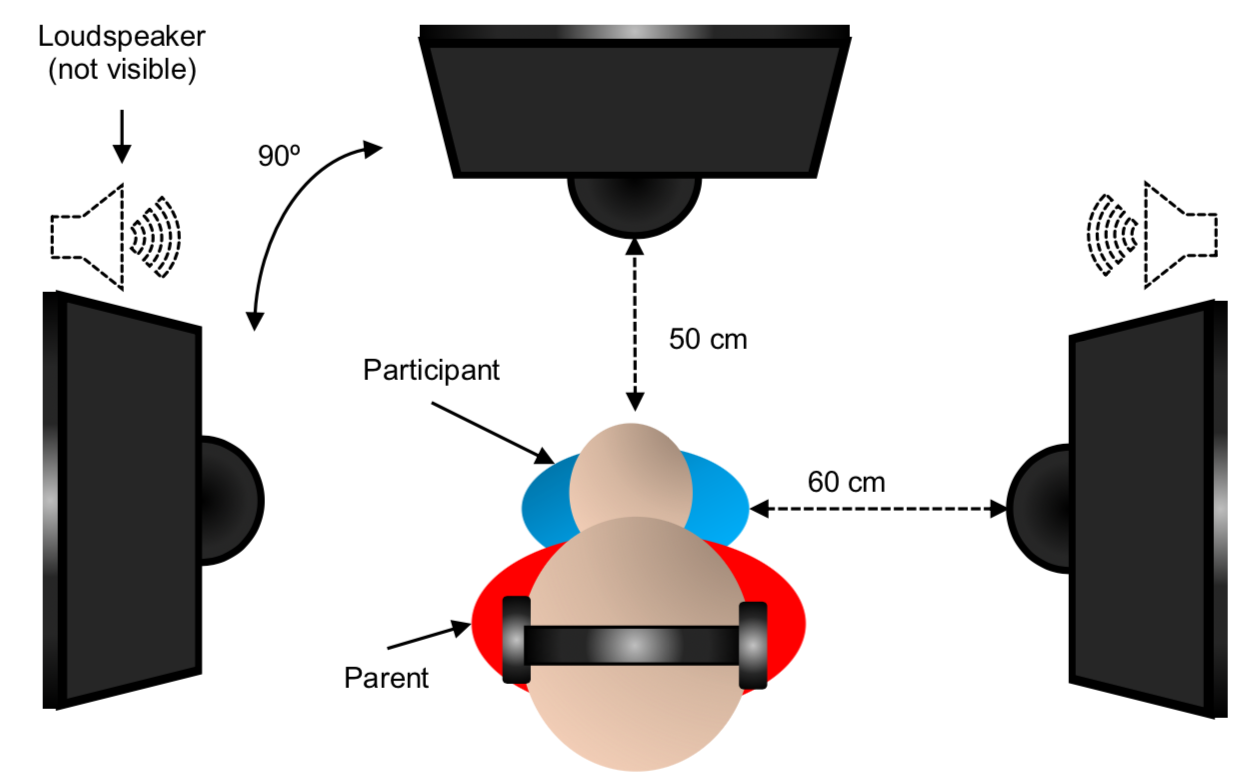
\includegraphics[width=1\linewidth]{/Users/GonzaloGGC/projects/Segmentation/Figures/setup} \caption{Aerial view of the experimental setup. Infants were sited in their parents' lap facing the central screen, with two screens located 90º at right and left from the central screen. Two loudspeakers (located next to the side screens played the acoustic stimuli. Both loudspeakers were hidden behind a white curtain.}\label{fig:hpp}
\end{figure}

To control potential intrinsic preferences towards any of the target words, half of the infants of both monolingual and bilingual groups were familiarized with \emph{gon} and \emph{mus} passages (condition \emph{gon-mus}) whereas the other half were familiarized with \emph{for} and \emph{pul} passages (condition \emph{for-pul}). All infants were tested with the four words. The parent was instructed not to interact with the infant during the whole procedure (e.g., no talking, pointing) and not to look to the side screens in order to avoid the infant to follow the parent's gaze. The parent wore noise-cancellation headphones playing loud music that masked the experimental speech stimuli. Figure 3 illustrates the procedure and design.

\begin{figure}
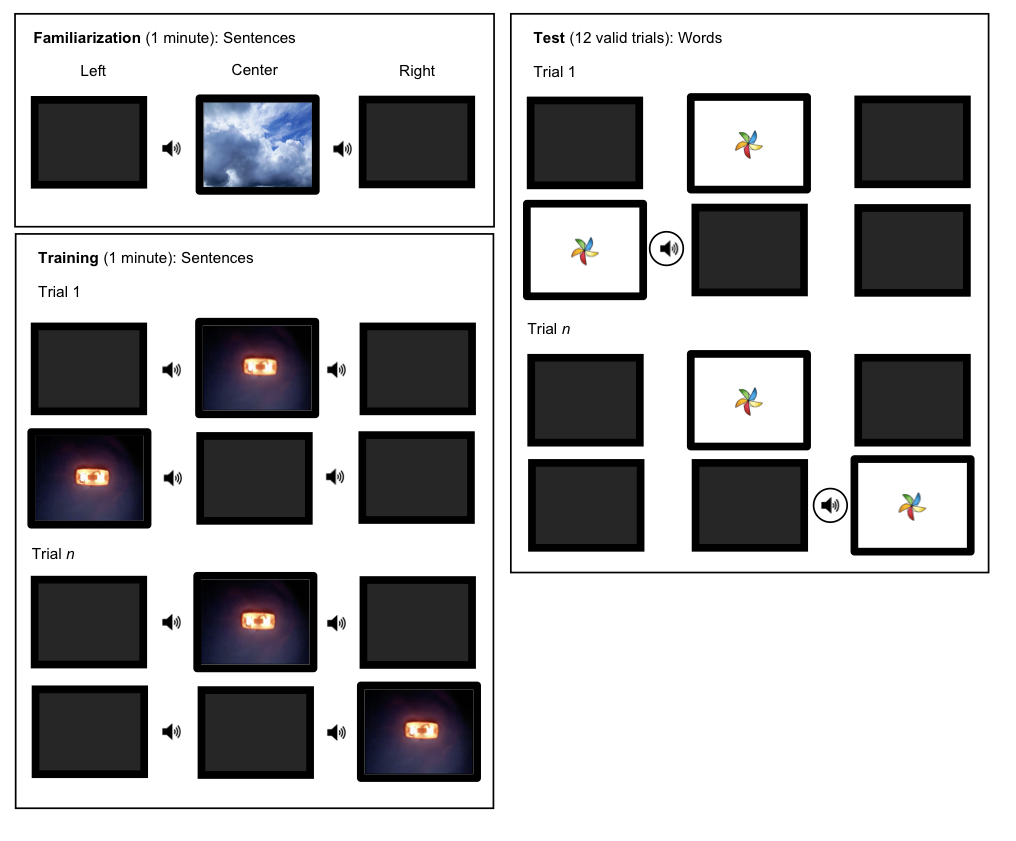
\includegraphics[width=1\linewidth]{/Users/GonzaloGGC/projects/Segmentation/Figures/procedure} \caption{Visual representation of the Head-turn Preference Procedure used (see Procedure section).}\label{fig:procedure}
\end{figure}

\hypertarget{familiarisation-phase}{%
\subsubsection{Familiarisation phase}\label{familiarisation-phase}}

We created a passage of 6 sentences embedding each word. Infants were familiarised with passages corresponding to two of the words. Hence, infants listened to two passages, what means that each infant listened to 12 different sentences, 6 embedding one word, 6 embedding the other word. The duration of each passage was similar. All infants listened to the sentences for 2 minutes. The duration of familiarisation was set according to Bosch and Sebastian-Galles (2003). During the first minute of familiarisation, infants listened to both passages of sentences (each embedding a target word) while moving clouds were displayed in the central screen. To control any intrinsic preference toward any of the words (which may potential bias looking preferences in the test phase), we counterbalanced the familiarisation words. Half of the infants were familiarised with the words \emph{gon} and \emph{mus} (condition \emph{gon-mus}), whereas the other half was familliarised with the words \emph{for} and \emph{pul} (condition \emph{for-pul}).

\hypertarget{training-phase}{%
\subsubsection{Training phase}\label{training-phase}}

During the second minute of familiarisation, infants listened agains both passages of sentences. This time, a blinking light was displayed in the central screen. When the infant fixated the blinking light, the light disappeared from the central screen and started being displayed in either the right or the left screen randomily. When the infant fixated the blinking light in the side screen at least once and stopped looking at it for at least 2 seconds, the light returned to the central screen. The aim of this minute of familiarisation is to alow infants to get used to make head turns towards the side screens.

\hypertarget{test-phase}{%
\subsubsection{Test phase}\label{test-phase}}

In the test phase, 12 trials were performed (3 for each of the 4 words). Three blocks of 12 trials were prepared. Words were separated by 2 seconds and repeated continuously in each trial until maximum of 18 seconds in each trials (7 repetitions max.). Each trial of the test phase consisted of repetitions of the same word. Words within the same trial were separated by 1,500 ms as in Bosch et al. (2013). Each trial started with the display of a rotating pinwheel in the central screen. When the infant looked at it, the stimulus disappeared and another one appeared in one of the side screens. A list of a random word was played from the loudspeaker in the same side. Listening time of each trial was registered. Orientation time towards the side in which stimuli were displayed was considered as listening time.

For the completion of the complete trial, a minimum of 2,000 ms of looking time was set. If visual orientation towards the screen was interrupted, recording time was paused and resumed once visual contact was re-established. After 2,000 ms of ceased visual orientation, the trial was stopped, and a new trial began. No predictions were made about the direction of preference towards the familiar or unfamiliar stimuli.

\hypertarget{results}{%
\section{Results}\label{results}}

As dependent variable, we measured looking time to the side screens for familiar and novel words presented at test. Differences in looking time for test words were considered as indicator of discrimination. Looking times in familiar and novel trials were aggregated for each participant by computing the mean looking time for the trials of each condition. Figure 4 shows looking times in novel and familiar trials by participant. A table presenting participant-level looking times is presented in Appendix 2.

\begin{figure}
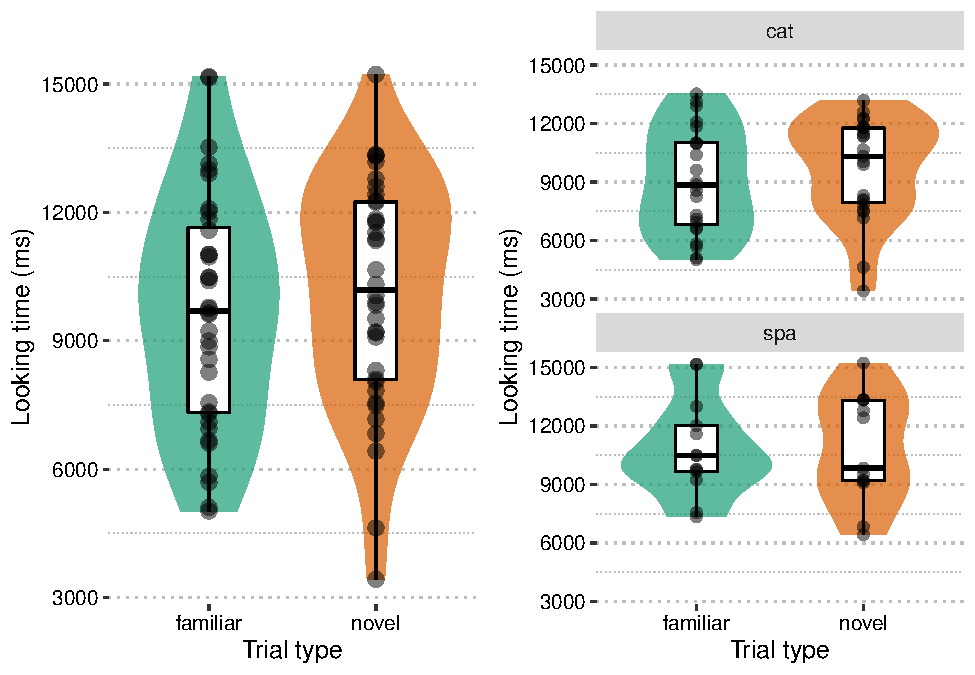
\includegraphics[width=1\linewidth]{segmentation_manuscript_files/figure-latex/unnamed-chunk-2-1} \caption{Looking time to familiar and unfamiliar words at test, overall and split by testing language. Boxplots represent the median, 25th and 75th percentiles. Contours represent the probability distribution.}\label{fig:unnamed-chunk-2}
\end{figure}

A paired \emph{t}-test comparing novel (\emph{Mean} = 10,110.31, \emph{SEM} = 445.25) and familiar (\emph{Mean} = 9,686.12, \emph{SEM} = 455.04) looking times failed to reject the null hypothesis at 0.05 significant criterion, \emph{t}(35) = 1.00, \emph{p} = .326, Cohen's \emph{d} = 0.12. A visual inspection of the data revealed that such a lack of statistically significant differences was unlikely to be due to the looking pattern of infants tested in a specific language. Given that this test does not provide any evidence supporting the null hypothesis, we opted to follow-up this analysis with equivalence testing. We performed two one-sided paired \emph{t}-tests, contrasting our \emph{t} estimate against those corresponding to the lower and upper threshold of the smallest effect size we are interested in detecting with our design. We defined such effect size as a Cohen's \emph{d} of 0.50. We based our decision in the most similar previous study we could find: Bosch et al. (2013) tested word segmentation from natural speech using a similar procedure in Catalan and Spanish monolinguals and bilinguals. The effect sizes of the contrasts comparing novel and familiar looking times approximated a Cohen's \emph{d} of 0.5 in all groups: \emph{d} = 0.41 for Spanish monolinguals, \emph{d} = 0.48 for Catalan monolinguals, and \emph{d} = 0.51 for Catalan-Spanish bilinguals. To perform this test, we used the TOSTER R package Lakens (2017). We achieved a statistical power of 82.50\% for both constrasts. Results are summarised in Table 1:

\begin{table}[tbp]
\begin{center}
\begin{threeparttable}
\caption{\label{tab:tost}Equivalence testing results.}
\begin{tabular}{ccccc}
\toprule
Test & t-value & df & p & Cohen's d\\
\midrule
t-test & -1.00 & 35 & .326 & -0.12\\
TOST Upper & -4.00 & 35 & < .001 & -0.47\\
TOST Lower & 2.00 & 35 & .026 & 0.24\\
\bottomrule
\end{tabular}
\end{threeparttable}
\end{center}
\end{table}

\begin{figure}
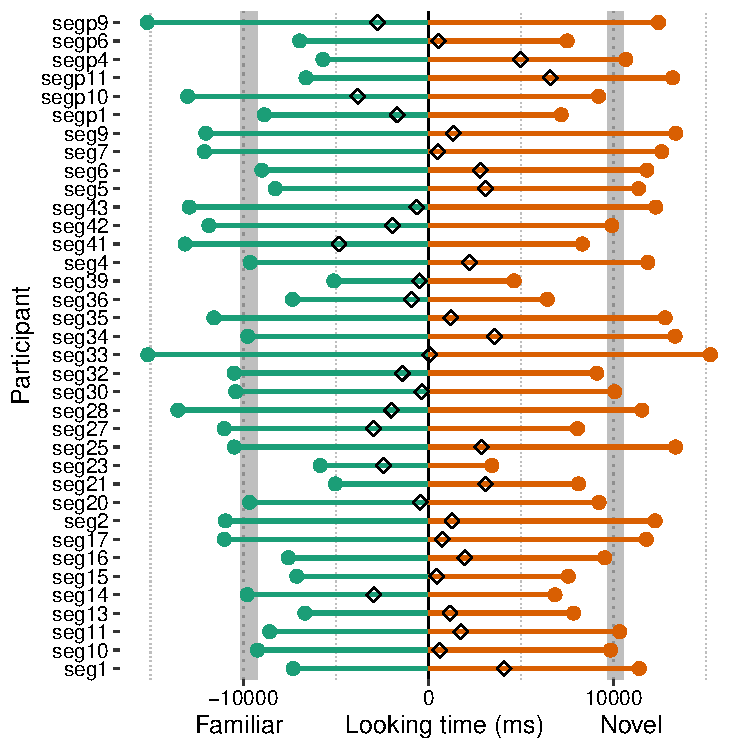
\includegraphics[width=1\linewidth]{segmentation_manuscript_files/figure-latex/unnamed-chunk-3-1} \caption{Looking time by trial type, and difference score by participant. Diamonds represent the difference score (Novel-Familiar). Grey shaded areas represent the mean and standard error of the mean for each trial type}\label{fig:unnamed-chunk-3}
\end{figure}

\hypertarget{acknowledgements}{%
\section{Acknowledgements}\label{acknowledgements}}

We thank Katia Pistrin, Xavier Mayoral and Silvia Blanch for their technical support, Alba Portet and Maria Coll for their help testing infants, Julia Monte for her help recording the stimuli, and the Speech Acquisition and Perception (SAP) research group members for their valuable comments on this manuscript. We also would like to thank all the parents and infants who so generously participated in this research.

\hypertarget{references}{%
\section{References}\label{references}}

\begingroup
\setlength{\parindent}{-0.5in}
\setlength{\leftskip}{0.5in}

\hypertarget{refs}{}
\leavevmode\hypertarget{ref-abboub2016}{}%
Abboub, N., Nazzi, T., \& Gervain, J. (2016). Prosodic grouping at birth. \emph{Brain and Language}, \emph{162}, 46--59. doi:\href{https://doi.org/10.1016/j.bandl.2016.08.002}{10.1016/j.bandl.2016.08.002}

\leavevmode\hypertarget{ref-albaredacastellot2011}{}%
Albareda-Castellot, B., Pons, F., \& Sebastian-Galles, N. (2011). The acquisition of phonetic categories in bilingual infants: New data from an anticipatory eye movement paradigm. \emph{Developmental Science}, \emph{14}(2), 395--401. doi:\href{https://doi.org/10.1111/j.1467-7687.2010.00989.x}{10.1111/j.1467-7687.2010.00989.x}

\leavevmode\hypertarget{ref-alcina1979}{}%
Alcina, J., Franch, J. A., \& Blecua, J. M. (1979). \emph{Gramatica espanola}. Ariel. Retrieved from \url{https://books.google.es/books?id=7nz8nQEACAAJ}

\leavevmode\hypertarget{ref-aslin1981}{}%
Aslin, R. N., Pisoni, D. B., Hennessy, B. L., \& Perey, A. J. (1981). Discrimination of voice onset time by human infants: new findings and implications for the effects of early experience. \emph{Child Development}, \emph{52}(4), 1135--1145. doi:\href{https://doi.org/10.1111/j.1467-8624.1981.tb03159.x}{10.1111/j.1467-8624.1981.tb03159.x}

\leavevmode\hypertarget{ref-bergmann2016}{}%
Bergmann, C., \& Cristia, A. (2016). Development of infants' segmentation of words from native speech: a meta-analytic approach. \emph{Developmental Science}, \emph{19}(6), 901--917. doi:\href{https://doi.org/10.1111/desc.12341}{10.1111/desc.12341}

\leavevmode\hypertarget{ref-bertoncini1995}{}%
Bertoncini, J., Floccia, C., Nazzi, T., \& Mehler, J. (1995). Basis o f Speech Representations in Neonates. \emph{Language and Speech}, \emph{38}(4), 311--329.

\leavevmode\hypertarget{ref-best2003}{}%
Best, C. T., \& McRoberts, G. W. (2003). Infant Perception of Non-Native Consonant Contrasts that Adults Assimilate in Different Ways. \emph{Language and Speech}, \emph{46}(2-3), 183--216. doi:\href{https://doi.org/10.1177/00238309030460020701}{10.1177/00238309030460020701}

\leavevmode\hypertarget{ref-best2001}{}%
Best, C. T., McRoberts, G. W., \& Goodell, E. \&. (2001). Discrimination of non-native consonant contrasts varying in perceptual assimilation to the listener's native phonological system. \emph{Journal of the Acoustical Society of America}, \emph{109}(2), 775--794. doi:\href{https://doi.org/10.1121/1.1332378}{10.1121/1.1332378}

\leavevmode\hypertarget{ref-best1995}{}%
Best, C. T., McRoberts, G. W., LaFleur, R., \& Silver-Isenstadt, J. (1995). Divergent developmental pattern for infants'perception of two non native consonant contrasts. \emph{Infant Behavior and Development}, \emph{18}, 339--350.

\leavevmode\hypertarget{ref-best1988}{}%
Best, C. T., McRoberts, G. W., \& Sithole, N. M. \&. (1988). Examination of perceptual reorganization for nonnative speech contrasts: Zulu click discrimination by English-speaking adults and infants. \emph{Journal of Experimental Psychology: Human Perception and Performance}, \emph{14}(3), 345--360. doi:\href{https://doi.org/10.1037/0096-1523.14.3.345}{10.1037/0096-1523.14.3.345}

\leavevmode\hypertarget{ref-bhatara2013}{}%
Bhatara, A., Boll-Avetisyan, N., Unger, A., Nazzi, T., \& Höhle, B. (2013). Native language affects rhythmic grouping of speech. \emph{The Journal of the Acoustical Society of America}, \emph{134}(5), 3828--3843. doi:\href{https://doi.org/10.1121/1.4823848}{10.1121/1.4823848}

\leavevmode\hypertarget{ref-praat}{}%
Boersma, P., \& Weenink, D. (2018). Praat: doing phonetics by computer {[}Computer program{]}. Retrieved from \url{http://www.praat.org/}

\leavevmode\hypertarget{ref-bosch2013}{}%
Bosch, L., Figueras, M., Teixidó, M., \& Ramon-Casas, M. (2013). Rapid gains in segmenting fluent speech when words match the rhythmic unit: Evidence from infants acquiring syllable-timed languages. \emph{Frontiers in Psychology}, \emph{4}(106), 1--12. doi:\href{https://doi.org/10.3389/fpsyg.2013.00106}{10.3389/fpsyg.2013.00106}

\leavevmode\hypertarget{ref-bosch2001}{}%
Bosch, L., \& Sebastian-Galles, N. (2001). Evidence of Early Language Discrimination Abilities in Infants From Bilingual Environments. \emph{Infancy}, \emph{2}(1), 29--49. doi:\href{https://doi.org/10.1207/S15327078IN0201_3}{10.1207/S15327078IN0201\_3}

\leavevmode\hypertarget{ref-bosch2003}{}%
Bosch, L., \& Sebastian-Galles, N. (2003). Simultaneous Bilingualism and the Perception of a Language-Specific Vowel Contrast in the First Year of Life. \emph{Language and Speech}, \emph{46}(2-3), 217--243. doi:\href{https://doi.org/10.1177/00238309030460020801}{10.1177/00238309030460020801}

\leavevmode\hypertarget{ref-christophe2001}{}%
Christophe, A., Mehler, J., \& Sebastian-Galles, N. (2001). Perception of Prosodic Boundary Correlates by Newborn Infants. \emph{Infancy}, \emph{2}(3), 385--394. doi:\href{https://doi.org/http://dx.doi.org/10.1207/S15327078IN0203_6}{http://dx.doi.org/10.1207/S15327078IN0203\_6}

\leavevmode\hypertarget{ref-dar2018}{}%
Dar, M., Keren-Portnoy, T., \& Vihman, M. M. (2018). An order effect in English infants' discrimination of an Urdu affricate contrast. \emph{Journal of Phonetics}, \emph{67}, 49--64. doi:\href{https://doi.org/10.1016/j.wocn.2017.12.002}{10.1016/j.wocn.2017.12.002}

\leavevmode\hypertarget{ref-decasper1986}{}%
DeCasper, A. J., \& Spence, M. J. (1986). Prenatal maternal speech influences newborns' perception of speech sounds. \emph{Infant Behavior and Development}, \emph{9}(2), 133--150. doi:\href{https://doi.org/10.1016/0163-6383(86)90025-1}{10.1016/0163-6383(86)90025-1}

\leavevmode\hypertarget{ref-dehaenelambertz1994}{}%
Dehaene-Lambertz, G., \& Dehaene, S. (1994). Speed and cerebral correlates of syllable discrimination in infants. \emph{Nature}, \emph{370}, 292--295.

\leavevmode\hypertarget{ref-dillon2013}{}%
Dillon, B., Dunbar, E., \& Idsardi, W. (2013). A Single-Stage approach to learning phonological categories: Insights from Inuktitut. \emph{Cognitive Science}, \emph{37}(2), 344--377. doi:\href{https://doi.org/10.1111/cogs.12008}{10.1111/cogs.12008}

\leavevmode\hypertarget{ref-eimas1971}{}%
Eimas, P. D., Siqueland, E. R., Jusczyk, P., \& Vigorito, J. (1971). Speech perception in infants. \emph{Science}, \emph{171}(3968), 303--306. doi:\href{https://doi.org/10.1126/science.171.3968.303}{10.1126/science.171.3968.303}

\leavevmode\hypertarget{ref-elsner2013}{}%
Elsner, M., Feldman, N. H., \& Wood, F. (2013). A Joint Learning Model of Word Segmentation, Lexical Acquisition, and Phonetic Variability. \emph{Proceedings of the 2013 Conference on Empirical Methods in Natural Language Processing}, 42--54.

\leavevmode\hypertarget{ref-feldman2013b}{}%
Feldman, N. H., Griffiths, T. L., Goldwater, S., \& Morgan, J. L. (2013a). A role for the developing lexicon in phonetic category acquisition. \emph{Psychological Review}, \emph{120}(4), 1--55. doi:\href{https://doi.org/10.1037/a0034245.A}{10.1037/a0034245.A}

\leavevmode\hypertarget{ref-feldman2013a}{}%
Feldman, N. H., Myers, E. B., White, K. S., Griffiths, T. L., \& Morgan, J. L. (2013b). Word-level information influences phonetic learning in adults and infants. \emph{Cognition}, \emph{127}(3), 427--438. doi:\href{https://doi.org/http://dx.doi.org/10.1016/j.cognition.2013.02.007}{http://dx.doi.org/10.1016/j.cognition.2013.02.007}

\leavevmode\hypertarget{ref-friederici2017}{}%
Friederici, A. D., Chomsky, N., Berwick, R. C., Moro, A., \& Bolhuis, J. J. (2017). Language, mind and brain. \emph{Nature Human Behaviour}, \emph{1}, 713--722. doi:\href{https://doi.org/10.1038/s41562-017-0184-4}{10.1038/s41562-017-0184-4}

\leavevmode\hypertarget{ref-friederici1993}{}%
Friederici, A. D., \& Wessels, J. M. I. (1993). Phonotactic knowledge of word boundaries and its use in infant speech perception. \emph{Perception \& Psychophysics}, \emph{54}(3), 287--295. doi:\href{https://doi.org/10.3758/BF03205263}{10.3758/BF03205263}

\leavevmode\hypertarget{ref-gonzalezgomez2013}{}%
Gonzalez-Gomez, N., \& Nazzi, T. (2013). Effects of Prior Phonotactic Knowledge on Infant Word Segmentation: The Case of Nonadjacent Dependencies. \emph{Journal of Speech, Language and Hearing Research}, \emph{56}(3), 840--849.

\leavevmode\hypertarget{ref-goyet2013}{}%
Goyet, L., Nishibayashi, L.-L., \& Nazzi, T. (2013). Early syllabic segmentation of fluent speech by infants acquiring French. \emph{PLoS ONE}, \emph{8}(11), 1--10. doi:\href{https://doi.org/10.1371/journal.pone.0079646}{10.1371/journal.pone.0079646}

\leavevmode\hypertarget{ref-green1988}{}%
Green, J. N. (1988). Spanish. In M. Harris \& N. Vincent (Eds.), \emph{The romance languages} (pp. 79--130). Cambrigde University Press.

\leavevmode\hypertarget{ref-houstonprice2004}{}%
Houston-Price, C., \& Nakai, S. (2004). Distinguishing novelty and familiarity effects in infant preference procedures. \emph{Infant and Child Development}, \emph{13}(4), 341--348. doi:\href{https://doi.org/10.1002/icd.364}{10.1002/icd.364}

\leavevmode\hypertarget{ref-hunter1988}{}%
Hunter, M. A., \& Ames, E. W. (1988). A multifactor model of infant preferences for novel and familiar stimuli. \emph{Advances in Infancy Research}, \emph{5}, 69--95.

\leavevmode\hypertarget{ref-jusczyk1995}{}%
Jusczyk, P. W., \& Aslin, R. N. (1995). Infants' Detection of the Sound Patterns of Words in Fluent Speech, \emph{29}(1), 1--23. doi:\href{https://doi.org/10.1006/cogp.1995.1010}{10.1006/cogp.1995.1010}

\leavevmode\hypertarget{ref-jusczyk1999}{}%
Jusczyk, P. W., Houston, D. M., \& Newsome, M. (1999). The beginnings of word segmentation in english-learning infants. \emph{Cognitive Psychology}, \emph{39}(3-4), 159--207. doi:\href{https://doi.org/10.1006/cogp.1999.0716}{10.1006/cogp.1999.0716}

\leavevmode\hypertarget{ref-kuhl2006}{}%
Kuhl, P. K., Stevens, E., Hayashi, A., Deguchi, T., Kiritani, S., \& Iverson, P. (2006). Infants show a facilitation effect for native language phonetic perception between 6 and 12 months. \emph{Developmental Science}, \emph{9}(2), 13--21. doi:\href{https://doi.org/10.1111/j.1467-7687.2006.00468.x}{10.1111/j.1467-7687.2006.00468.x}

\leavevmode\hypertarget{ref-kuhl1992}{}%
Kuhl, P. K., Williams, K. A., Lacerda, F., Stevens, K. N., \& Lindblom, B. (1992). Linguistic experience alters phonetic perception in infants by 6 months of age. \emph{Science}, \emph{255}(5), 606--608.

\leavevmode\hypertarget{ref-lakens2017}{}%
Lakens, D. (2017). Equivalence tests: A practical primer for t-tests, correlations, and meta-analyses. \emph{Social Psychological and Personality Science}, \emph{1}, 1--8. doi:\href{https://doi.org/10.1177/1948550617697177}{10.1177/1948550617697177}

\leavevmode\hypertarget{ref-marimon2015}{}%
Marimon, M. (2015). \emph{Is the lexicon affecting early word segmentation? A segmentation task at 8 months of age} (PhD thesis). Universitat Pompeu Fabra.

\leavevmode\hypertarget{ref-mattys2001}{}%
Mattys, S. L., \& Jusczyk, P. W. (2001). Phonotactic cues for segmentation of fluent speech by infants. \emph{Cognition}, \emph{78}(2), 91--121. doi:\href{https://doi.org/https://doi.org/10.1016/S0010-0277(00)00109-8}{https://doi.org/10.1016/S0010-0277(00)00109-8}

\leavevmode\hypertarget{ref-may2011}{}%
May, L., Byers-Heinlein, K., Gervain, J., \& Werker, J. F. (2011). Language and the newborn brain: does prenatal language experience shape the neonate neural response to speech? \emph{Frontiers in Psychology}, \emph{2}, 222. doi:\href{https://doi.org/http://dx.doi.org/10.3389/fpsyg.2011.00222}{http://dx.doi.org/10.3389/fpsyg.2011.00222}

\leavevmode\hypertarget{ref-maye2008}{}%
Maye, J., Weiss, D. J., \& Aslin, R. N. (2008). Statistical phonetic learning in infants: Facilitation and feature generalization. \emph{Developmental Science}, \emph{11}(1), 122--134. doi:\href{https://doi.org/http://dx.doi.org/10.1111/j.1467-7687.2007.00653.x}{http://dx.doi.org/10.1111/j.1467-7687.2007.00653.x}

\leavevmode\hypertarget{ref-maye2002}{}%
Maye, J., Werker, J. F., \& Gerken, L. (2002). Infant sensitivity to distributional information can affect phonetic discrimination. \emph{Cognition}, \emph{82}(3), 101--111. doi:\href{https://doi.org/http://dx.doi.org/10.1016/S0010-0277(01)00157-3}{http://dx.doi.org/10.1016/S0010-0277(01)00157-3}

\leavevmode\hypertarget{ref-mersad2012}{}%
Mersad, K., \& Nazzi, T. (2012). When Mommy Comes to the Rescue of Statistics: Infants Combine Top-Down and Bottom-Up Cues to Segment Speech. \emph{Language Learning and Development}, \emph{8}(3), 303--315. doi:\href{https://doi.org/http://dx.doi.org/10.1080/15475441.2011.609106}{http://dx.doi.org/10.1080/15475441.2011.609106}

\leavevmode\hypertarget{ref-moon2013}{}%
Moon, C. M., Lagercrantz, H., \& Kuhl, P. K. (2013). Language experienced in utero affects vowel perception after birth: A two-country study. \emph{Acta Paediatrica}, \emph{102}(2), 156--160. doi:\href{https://doi.org/10.1111/apa.12098}{10.1111/apa.12098}

\leavevmode\hypertarget{ref-nazzi2005}{}%
Nazzi, T., Dilley, L. C., Jusczyk, A. M., Shattuck-Hufnagel, S., \& Jusczyk, P. W. (2005). English-Learning Infants' Segmentation of Verbs from Fluent Speech. \emph{Language and Speech}, \emph{48}(3), 279--298. doi:\href{https://doi.org/http://dx.doi.org/10.1177/00238309050480030201}{http://dx.doi.org/10.1177/00238309050480030201}

\leavevmode\hypertarget{ref-nishibayashi2015}{}%
Nishibayashi, L.-L., Goyet, L., \& Nazzi, T. (2015). Early Speech Segmentation in French-Learning Infants: Monosyllabic Words versus Embedded Syllables. \emph{Language and Speech}, \emph{58}(3), 334--350. doi:\href{https://doi.org/http://dx.doi.org/10.1177/0023830914551375}{http://dx.doi.org/10.1177/0023830914551375}

\leavevmode\hypertarget{ref-polka1996}{}%
Polka, L., \& Bohn, O. (1996). A cross‐language comparison of vowel perception in English‐learning and German‐learning infants. \emph{The Journal of the Acoustical Society of America}, \emph{100}(1), 577--592. doi:\href{https://doi.org/10.1121/1.415884}{10.1121/1.415884}

\leavevmode\hypertarget{ref-polka2001}{}%
Polka, L., Colantonio, C., \& Sundara, M. (2001). A cross-language comparison of /d /--/d-th/ perception: Evidence for a new developmental pattern. \emph{The Journal of the Acoustical Society of America}, \emph{109}(5), 2190--2201. doi:\href{https://doi.org/10.1121/1.1362689}{10.1121/1.1362689}

\leavevmode\hypertarget{ref-polka2017}{}%
Polka, L., Orena, A. J., Sundara, M., \& Worrall, J. (2017). Segmenting words from fluent speech during infancy -- challenges and opportunities in a bilingual context. \emph{Developmental Science}, \emph{20}(1), 1--14. doi:\href{https://doi.org/10.1111/desc.12419}{10.1111/desc.12419}

\leavevmode\hypertarget{ref-polka1994}{}%
Polka, L., \& Werker, J. F. (1994). Developmental changes in perception of nonnative vowel contrasts. \emph{Journal of Experimental Psychology: Human Perception and Performance}, \emph{20}(2), 421--435. doi:\href{https://doi.org/http://dx.doi.org/10.1037/0096-1523.20.2.421}{http://dx.doi.org/10.1037/0096-1523.20.2.421}

\leavevmode\hypertarget{ref-rafel1979}{}%
Rafel, J. (1979). Dades sobre la frequencia de les unitats fonologiques en catala. \emph{Estudis Universitaris Catalans}, \emph{23}(2), 473--496.

\leavevmode\hypertarget{ref-ramoncasas2017}{}%
Ramon-Casas, M., Fennell, C. T., \& Bosch, L. (2017). Minimal-pair word learning by bilingual toddlers: The Catalan /e/-/epsilon/ contrast revisited. \emph{Bilingualism}, \emph{20}(3), 649--656. doi:\href{https://doi.org/10.1017/S1366728916001115}{10.1017/S1366728916001115}

\leavevmode\hypertarget{ref-ramoncasas2009}{}%
Ramon-Casas, M., Swingley, D., Sebastian-Galles, N., \& Bosch, L. (2009). Vowel categorization during word recognition in bilingual toddlers. \emph{Cognitive Psychology}, \emph{59}(1), 96--121. doi:\href{https://doi.org/http://dx.doi.org/10.1016/j.cogpsych.2009.02.002}{http://dx.doi.org/10.1016/j.cogpsych.2009.02.002}

\leavevmode\hypertarget{ref-saffran1996}{}%
Saffran, J. R., Aslin, R. N., \& Newport, E. L. (1996). Statistical learning by 8-month-old infants. \emph{Science}, \emph{274}(5294), 1926--1928. doi:\href{https://doi.org/http://dx.doi.org/10.1126/science.274.5294.1926}{http://dx.doi.org/10.1126/science.274.5294.1926}

\leavevmode\hypertarget{ref-saffran2018}{}%
Saffran, J. R., \& Kirkham, N. Z. (2018). Infant Statistical Learning. \emph{Annual Review of Psychology}, \emph{69}(2), 1--23. doi:\href{https://doi.org/10.1146/annurev-psych-122216-011805}{10.1146/annurev-psych-122216-011805}

\leavevmode\hypertarget{ref-santolin2018}{}%
Santolin, C., \& Saffran, J. R. (2018). Constraints on Statistical Learning Across Species. \emph{Trends in Cognitive Sciences}, \emph{22}(1), 52--63. doi:\href{https://doi.org/10.1016/j.tics.2017.10.003}{10.1016/j.tics.2017.10.003}

\leavevmode\hypertarget{ref-sebastiangalles2002}{}%
Sebastian-Galles, N., \& Bosch, L. (2002). Building phonotactic knowledge in bilinguals: Role of early exposure. \emph{Journal of Experimental Psychology: Human Perception and Performance}, \emph{28}(4), 974--989. doi:\href{https://doi.org/http://dx.doi.org/10.1037/0096-1523.28.4.974}{http://dx.doi.org/10.1037/0096-1523.28.4.974}

\leavevmode\hypertarget{ref-sebastiangalles2009}{}%
Sebastian-Galles, N., \& Bosch, L. (2009). Developmental shift in the discrimination of vowel contrasts in bilingual infants: Is the distributional account all there is to it? \emph{Developmental Science}, \emph{12}(6), 874--887. doi:\href{https://doi.org/http://dx.doi.org/10.1111/j.1467-7687.2009.00829.x}{http://dx.doi.org/10.1111/j.1467-7687.2009.00829.x}

\leavevmode\hypertarget{ref-segal2016}{}%
Segal, O., Hejli-Assi, S., \& Kishon-Rabin, L. (2016). The effect of listening experience on the discrimination of /ba/ and /pa/ in Hebrew-learning and Arabic-learning infants. \emph{Infant Behavior and Development}, \emph{42}, 86--99. doi:\href{https://doi.org/10.1016/j.infbeh.2015.10.002}{10.1016/j.infbeh.2015.10.002}

\leavevmode\hypertarget{ref-shin2018}{}%
Shin, M., Choi, Y., \& Mazuka, R. (2018). Development of fricative sound perception in Korean infants: The role of language experience and infants' initial sensitivity. \emph{PloS ONE}, \emph{13}(6), 1--12.

\leavevmode\hypertarget{ref-skoruppa2013}{}%
Skoruppa, K., Pons, F., Bosch, L., Christophe, A., Cabrol, D., \& Peperkamp, S. (2013). The Development of Word Stress Processing in French and Spanish Infants. \emph{Language Learning and Development}, \emph{9}(1), 88--104. doi:\href{https://doi.org/http://dx.doi.org/10.1080/15475441.2012.693881}{http://dx.doi.org/10.1080/15475441.2012.693881}

\leavevmode\hypertarget{ref-audacity}{}%
Team, A. (2018, December). Audacity(R): Free Audio Editor and Recorder {[}Computer application{]}. Retrieved from \href{https://audacityteam.org/\%20}{https://audacityteam.org/ }

\leavevmode\hypertarget{ref-thiessen2003}{}%
Thiessen, E. D., \& Saffran, J. R. (2003). When cues collide: Use of stress and statistical cues to word boundaries by 7- to 9-month-old infants. \emph{Developmental Psychology}, \emph{39}(4), 706--716. doi:\href{https://doi.org/10.1037/0012-1649.39.4.706}{10.1037/0012-1649.39.4.706}

\leavevmode\hypertarget{ref-tsuji2014}{}%
Tsuji, S., \& Cristia, A. (2014). Perceptual attunement in vowels: A meta‐analysis. \emph{Developmental Psychobiology}, \emph{56}(2), 179--191. doi:\href{https://doi.org/http://dx.doi.org/10.1002/dev.21179}{http://dx.doi.org/10.1002/dev.21179}

\leavevmode\hypertarget{ref-werker1981}{}%
Werker, J. F., Gilbert, J. H. V., Humphrey, K., \& Tees, R. C. (1981). Developmental aspects of cross-language speech perception. \emph{Child Development}, \emph{52}(1), 349--355. Retrieved from \url{http://www.jstor.org/stable/1129249}

\leavevmode\hypertarget{ref-werker1984}{}%
Werker, J. F., \& Tees, R. C. (1984). \emph{Infant Behavior \& Development}, \emph{7}(1), 49--63. doi:\href{https://doi.org/http://dx.doi.org/10.1016/S0163-6383(84)80022-3}{http://dx.doi.org/10.1016/S0163-6383(84)80022-3}

\leavevmode\hypertarget{ref-werker2002}{}%
Werker, J. F., \& Tees, R. C. (2002). Cross-language speech perception: Evidence for perceptual reorganization during the first year of life. \emph{Infant Behavior and Development}, \emph{25}(1), 121--133. doi:\href{https://doi.org/10.1016/S0163-6383(02)00093-0}{10.1016/S0163-6383(02)00093-0}

\leavevmode\hypertarget{ref-yoshida2010}{}%
Yoshida, K. A., Pons, F., Maye, J., \& Werker, J. F. (2010). Distributional phonetic learning at 10 months of age. \emph{Infancy}, \emph{15}(4), 420--433. doi:\href{https://doi.org/http://dx.doi.org/10.1111/j.1532-7078.2009.00024.x}{http://dx.doi.org/10.1111/j.1532-7078.2009.00024.x}

\endgroup


\end{document}
